\documentclass[12pt]{article}

\usepackage{tikz,pgf}
\usepackage{slashbox}
\usepackage{caption}
\usepackage{circuitikz}
\usetikzlibrary{automata, positioning}
\usetikzlibrary{shapes.gates.logic.US,shapes.gates.logic.IEC}

\usepackage{pgf}
\usepackage{verbatim}
%%%>

\usetikzlibrary{calc,arrows}
\usepackage{amsmath}

\makeatletter

% Data Flip Flip (DFF) shape
\pgfdeclareshape{dff}{
    % The 'minimum width' and 'minimum height' keys, not the content, determine
    % the size
    \savedanchor\northeast{%
        \pgfmathsetlength\pgf@x{\pgfshapeminwidth}%
        \pgfmathsetlength\pgf@y{\pgfshapeminheight}%
        \pgf@x=0.5\pgf@x
        \pgf@y=0.5\pgf@y
    }
    % This is redundant, but makes some things easier:
    \savedanchor\southwest{%
        \pgfmathsetlength\pgf@x{\pgfshapeminwidth}%
        \pgfmathsetlength\pgf@y{\pgfshapeminheight}%
        \pgf@x=-0.5\pgf@x
        \pgf@y=-0.5\pgf@y
    }
    % Inherit from rectangle
    \inheritanchorborder[from=rectangle]

    % Define same anchor a normal rectangle has
    \anchor{center}{\pgfpointorigin}
    \anchor{north}{\northeast \pgf@x=0pt}
    \anchor{east}{\northeast \pgf@y=0pt}
    \anchor{south}{\southwest \pgf@x=0pt}
    \anchor{west}{\southwest \pgf@y=0pt}
    \anchor{north east}{\northeast}
    \anchor{north west}{\northeast \pgf@x=-\pgf@x}
    \anchor{south west}{\southwest}
    \anchor{south east}{\southwest \pgf@x=-\pgf@x}
    \anchor{text}{
        \pgfpointorigin
        \advance\pgf@x by -.5\wd\pgfnodeparttextbox%
        \advance\pgf@y by -.5\ht\pgfnodeparttextbox%
        \advance\pgf@y by +.5\dp\pgfnodeparttextbox%
    }

    % Define anchors for signal ports
    \anchor{D}{
        \pgf@process{\northeast}%
        \pgf@x=-1\pgf@x%
        \pgf@y=.5\pgf@y%
    }
    \anchor{CLK}{
        \pgf@process{\northeast}%
        \pgf@x=-1\pgf@x%
        \pgf@y=-.66666\pgf@y%
    }
    \anchor{CE}{
        \pgf@process{\northeast}%
        \pgf@x=-1\pgf@x%
        \pgf@y=-0.33333\pgf@y%
    }
    \anchor{Q}{
        \pgf@process{\northeast}%
        \pgf@y=.5\pgf@y%
    }
    \anchor{Qn}{
        \pgf@process{\northeast}%
        \pgf@y=-.5\pgf@y%
    }
    \anchor{R}{
        \pgf@process{\northeast}%
        \pgf@x=0pt%
    }
    \anchor{S}{
        \pgf@process{\northeast}%
        \pgf@x=0pt%
        \pgf@y=-\pgf@y%
    }
    % Draw the rectangle box and the port labels
    \backgroundpath{
        % Rectangle box
        \pgfpathrectanglecorners{\southwest}{\northeast}
        % Angle (>) for clock input
        \pgf@anchor@dff@CLK
        \pgf@xa=\pgf@x \pgf@ya=\pgf@y
        \pgf@xb=\pgf@x \pgf@yb=\pgf@y
        \pgf@xc=\pgf@x \pgf@yc=\pgf@y
        \pgfmathsetlength\pgf@x{1.6ex} % size depends on font size
        \advance\pgf@ya by \pgf@x
        \advance\pgf@xb by \pgf@x
        \advance\pgf@yc by -\pgf@x
        \pgfpathmoveto{\pgfpoint{\pgf@xa}{\pgf@ya}}
        \pgfpathlineto{\pgfpoint{\pgf@xb}{\pgf@yb}}
        \pgfpathlineto{\pgfpoint{\pgf@xc}{\pgf@yc}}
        \pgfclosepath

        % Draw port labels
        \begingroup
            \tikzset{flip flop/port labels} % Use font from this style
            \tikz@textfont

            \pgf@anchor@dff@D
            \pgftext[left,base,at={\pgfpoint{\pgf@x}{\pgf@y}},x=\pgfshapeinnerxsep]{\raisebox{-0.75ex}{D}}

            \pgf@anchor@dff@CE
            \pgftext[left,base,at={\pgfpoint{\pgf@x}{\pgf@y}},x=\pgfshapeinnerxsep]{\raisebox{-0.75ex}{CE}}

            \pgf@anchor@dff@Q
            \pgftext[right,base,at={\pgfpoint{\pgf@x}{\pgf@y}},x=-\pgfshapeinnerxsep]{\raisebox{-.75ex}{Q}}

            \pgf@anchor@dff@Qn
            \pgftext[right,base,at={\pgfpoint{\pgf@x}{\pgf@y}},x=-\pgfshapeinnerxsep]{\raisebox{-.75ex}{$\overline{\mbox{Q}}$}}

            \pgf@anchor@dff@R
            \pgftext[top,at={\pgfpoint{\pgf@x}{\pgf@y}},y=-\pgfshapeinnerysep]{R}

            \pgf@anchor@dff@S
            \pgftext[bottom,at={\pgfpoint{\pgf@x}{\pgf@y}},y=\pgfshapeinnerysep]{S}
        \endgroup
    }
}

% Key to add font macros to the current font
\tikzset{add font/.code={\expandafter\def\expandafter\tikz@textfont\expandafter{\tikz@textfont#1}}}

% Define default style for this node
\tikzset{flip flop/port labels/.style={font=\sffamily\scriptsize}}
\tikzset{every dff node/.style={draw,minimum width=2cm,minimum
        height=2.828427125cm,very thick,inner sep=1mm,outer sep=0pt,cap=round,add
        font=\sffamily}}
\begin{document}

\begin{enumerate}
    \item
        The state diagram is like below:

        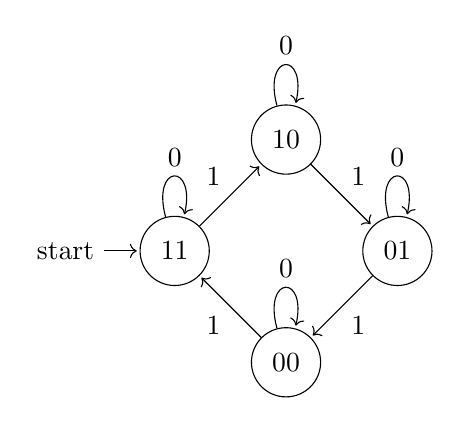
\begin{tikzpicture}[shorten >=1pt,node distance=2cm,on grid,auto]
            \node[state,initial] (11) {11};
            \node[state] (10) [above right=of 11] {10};
            \node[state] (00) [below right=of 11] {00};
            \node[state](01)  [above right=of 00] {01};
            \path [->]
            (11) edge node {1} (10)
            edge [loop above] node {0} ()
            (10) edge node {1} (01)
            edge [loop above] node {0} ()
            (01) edge node {1} (00)
            edge [loop above] node {0} ()
            (00) edge node {1} (11)
            edge [loop above] node {0} ();
        \end{tikzpicture}

        The state table is like the following:
        \begin{tabular}{c|cc}

            $x$ & Current State & Next State\\ \hline
            0 & 00 & 00\\
            0 & 01 & 01\\
            0 & 10 & 10\\
            0 & 11 & 11\\
            1 & 00 & 11\\
            1 & 01 & 00\\
            1 & 10 & 01\\
            1 & 11 & 10\\
        \end{tabular}

        \begin{table}[h]
            \centering
            \begin{tabular}{|c|c|c|c|c|}
                \hline
                \backslashbox{x}{Current State} & 00 & 01 & 11 & 10 \\ \hline
                0 &0&0&1&1\\ \hline
                1 &1&0&1&0\\ \hline

            \end{tabular}
            \captionof{table}{Karnugh Map for $D_1$}
        \end{table}
        \begin{table}[h]
            \centering
            \begin{tabular}{|c|c|c|c|c|}
                \hline
                \backslashbox{x}{Current State} & 00 & 01 & 11 & 10 \\ \hline
                0 &0&1&1&0\\ \hline
                1 &1&0&0&1\\ \hline

            \end{tabular}
            \captionof{table}{Karnugh Map for $D_2$}
        \end{table}
        The circuit is like below:


        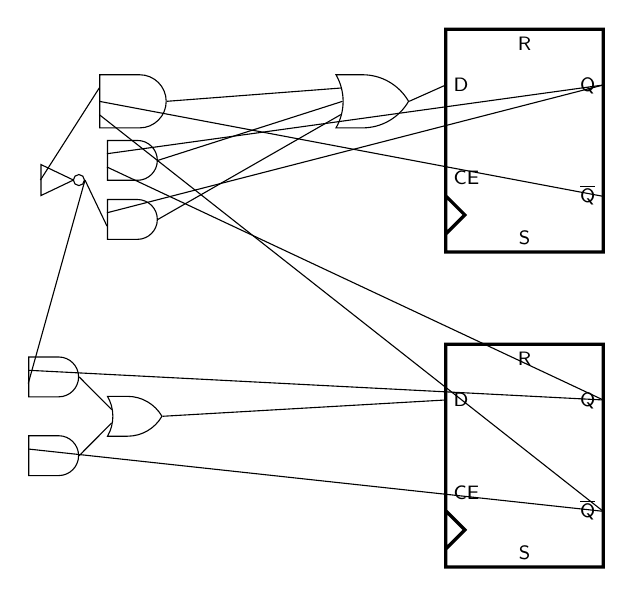
\begin{tikzpicture}[font=\sffamily,>=triangle 45]
            \node [shape=dff] (DFF0) at ( 6,0 ) {};
            \node [shape=dff] (DFF1) at ( 6,4 ) {};
            \node [not gate US, draw] at (0,3.5) (xnot) {};
            \node [and gate US, draw] at (1,3) (and1) {};
            \node [and gate US, draw] at (1,3.75) (and2) {};
            \node [and gate US, draw, logic gate inputs=nnn] at (1,4.5) (and3) {};
            \node [or gate US, draw, logic gate inputs=nnn] at (4,4.5) (or1) {};
            \node [and gate US, draw] at (0,0) (and4) {};
            \node [and gate US, draw] at (0,1) (and5) {};
            \node [or gate US, draw] at (1,0.5) (or2) {};
            %(xnot.in) node[anchor = east] {$x$}
            \draw (or1.output) -- (DFF1.D);
            \draw (DFF1.Q) -- (and1.input 1);
            \draw (xnot.output) -- (and1.input 2);
            \draw (DFF1.Q) -- (and2.input 1);
            \draw (DFF0.Q) -- (and2.input 2);
            \draw (xnot.input) -- (and3.input 1);
            \draw (DFF1.Qn) -- (and3.input 2);
            \draw (DFF0.Qn) -- (and3.input 3);
            \draw (and3.output) -- (or1.input 1);
            \draw (and2.output) -- (or1.input 2);
            \draw (and1.output) -- (or1.input 3);
            \draw (and4.output) -- (or2.input 2);
            \draw (and5.output) -- (or2.input 1);
            \draw (or2.output) -- (DFF0.D);
            \draw (DFF0.Qn) -- (and4.input 1);
            \draw (DFF0.Q) -- (and5.input 1);
            \draw (xnot.output) -- (and5.input 2);

        \end{tikzpicture}
    \item
        \begin{enumerate}
            \item
                1- Capacity of the memory.
                2- Speed of the memory.
                3- Cost of the memory.
            \item
                We use memory hierarchy to have the maximum capacity
                and speed and minimum cost. The method is that you use memories
                with higher speed in the place in which they are closer to the
                CPU and memories with less speed but more capacity further from
                the CPU. To have maximum speed and capacity and minimum cost.

            \item
                Yes, when the time of retrieving data from the intermediate
                memories is more than the time of retrieving data from the main
                memory.
            \item
                Static memories are more expensive and have high speed because
                they don't need refreshing and less dense and they use less power.
                But Dynamic memories are chipper but they need refresher and so
                they are slower than static memories and they are denser than
                static memories and they use more power. - Using static memories
                is easier.
        \end{enumerate}
    \item

        $T_{access}=t_1+(1-h_1)(t_2+(1-h_2)(t_3+(1-h_3)t)))=
        3*10^{-9}+0.08*(20*10^{-9}+0.25*(350*10^{-9}+0.65*12*10^{-3}))=1.56*10^{-4} s$
        \begin{enumerate}
            \item
                $T_{access}=t_1+(1-h_1)(t_2+(1-h_2)(t_3+(1-h_3)t)))=
                3*10^{-9}+0.08*(20*10^{-9}+0.30*(350*10^{-9}+0.65*12*10^{-3}))=1.87213*10^{-4}$


                It is 0.83 times slower than the first system.
            \item
                $T_{access}=t_1+(1-h_1)(t_2+(1-h_2)(t_3+(1-h_3)(t_4+1-h_4(t_5))))=
                3*10^{-9}+0.08*(8*10^{-9}+0.15*(20*10^{-9}+0.3*(10^{-9}*350+0.65*
                10^{-3}*12)))=2.81*10^{-5}$

                It is 5.551 times faster than the first system.
        \end{enumerate}
    \item
        \begin{enumerate}
            \item
                width = bitline = 8B = $8*8$ = 64 bits.\\
                height = wordline = 64 * 1024 = 65536 bits.\\
                volume = size = $64*65536$ = 4194304 bits.\\
                number of bits for addressing = $\log_2{65536}=16.0$
            \item
                width = bitline = 1B = $1*8$ = 8 bits.\\
                height = wordline = 16 * 1024 = 16384 bits.\\
                volume = size = $8*16384$ = 131072 bits.\\
                number of bits for addressing = $\log_2{131072}=17.0$
            \item
                width = bitline = 4B = $4*8$ = 32 bits.\\
                height = wordline = $2^{13}$ = 8192 bits.\\
                volume = size = $32*8192$ = 262144 bits.\\
                number of bits for addressing = 13 bits\\

        \end{enumerate}

\end{enumerate}

\end{document}
